\subsubsection{Tarjeta de almacenamiento SD}

Para incluir una tarjeta de almacenamiento SD en el sistema, se utilizó un zócalo modelo DM3AT-SF-PEJM5 de Hirose Connector \cite{DM3AT-SF-PEJM5}. Este conector admite tarjetas micro SD y tiene un sistema de \textit{push-pull} que permite manipular más fácilmente la colocación de la tarjeta. Para la tarjeta micro SD se utilizó el modelo Micro SD Ultra 8GB Clase 10 de Sandisk \cite{sd_sandisk} porque se reutilizó de otro proyecto. Sin embargo, al ser un componente de simple extracción y reemplazo, se considera que se debe utilizar una unidad de almacenaje de mayor memoria. \\

En la figura \ref{fig:sd_sch} se observa la conexión del circuito con el zócalo para micro SD. Se utilizó la interfaz SPI del MCU para la comunicación con la SD y se colocaron algunas resistencias de \textit{pull-up} recomendadas en los buses de datos o líneas desconectadas. También se incluyeron capacitores de desacople para reducir el ruido en la alimentación de la SD. El zócalo incluye además una conexión mecánica que permite determinar si existe una tarjeta colocada en el zócalo o no; esto se conecta con una entrada del MCU para poder considerar el estado físico real de la tarjeta. 



\begin{figure}[H]
    \centering
    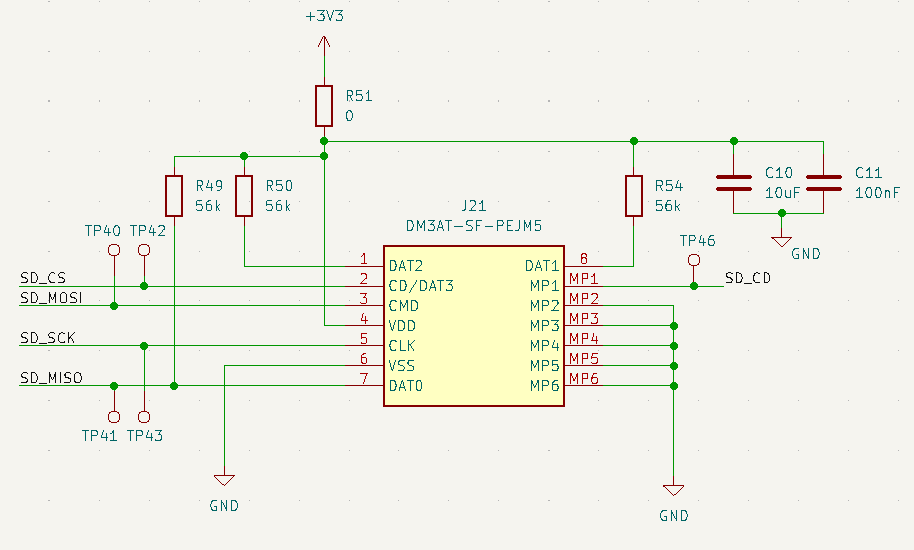
\includegraphics[width = \linewidth]{img/sd_sch.png}
    \caption{Circuito de conexión con la tarjeta SD}
    \label{fig:sd_sch}
\end{figure}    